%!TEX root = mainfile.tex

\section{Contaminants} % (fold)
\label{sec:contaminants}
    \subsection{Low Mass Stars} % (fold)
    \label{sub:low_mass_stars}
        These can easily be identified due to the high resolution imaging provided by \ldots. The Point-spread function (PSF) obtained will allow us to determine which sources are point-like and which are extended. We should be able to avoid significant contamination by removing any point-like sources from the results as all galaxies should have a great enough diameter.
    % subsection low_mass_stars (end)

    \subsection{Spurious Sources} % (fold)
    \label{sub:spurious_sources}
        By stipulating that we will be requiring detections in two bands the influence of spurious sources will be negligible. Finding detections in 2 bands at reasonable confidence interval (?3sig?) is very improbable. By inspecting the negative with the same requirements for detection we are able to identify any such sources easily\cite{Bouwens2011}.
    % subsection spurious_sources (end)

    \subsection{Supernovae and other transient sources} % (fold)
    \label{sub:supernovae_and_other_transient_sources}
        Events such as Supernovae happen incredibly quickly releasing a vast amount of energy, as seen in figure~\ref{fig:SNe_1987a}. These events can spoil images due to their short duration by introducing new data in only a portion of the sample. These effects are usually only considered when taking exposures years apart or when combining multiple sources over a long timescale. Such events are very unlikely to contaminate our results as we propose to take our images close in time.
        \begin{figure}[ht]
            \centering
            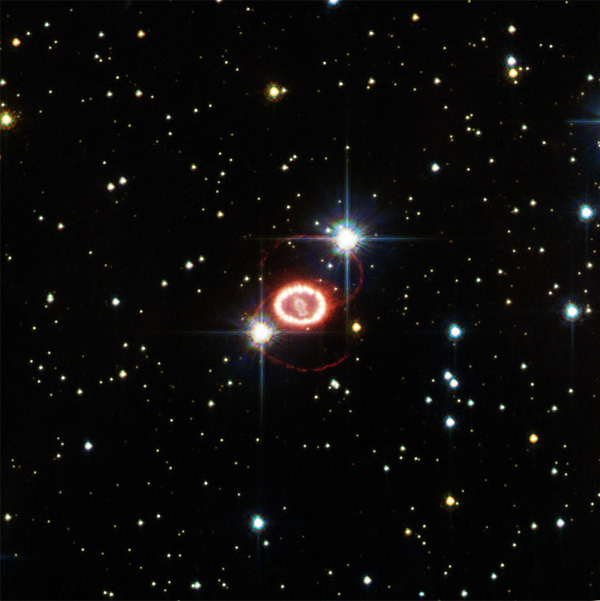
\includegraphics[width=0.6\textwidth]{../Images/SNe_1987a.jpg}
            \caption{The shockwave from Supernova 1987a imaged by HST in 2006.\label{fig:SNe_1987a}}
        \end{figure}
    % subsection supernovae_and_other_transient_sources (end)

    \subsection{Lower Redshift Sources and photometric scattering} % (fold)
    \label{sub:lower_redshift_sources_and_photometric_scattering}
        This category is likely to provide the greatest source of contamination for the surveyed area. It will do so increasingly at high redshifts where its affect on the faintest magnitudes is most greatly felt. Its affect is most influential with a small S/N ratio for the observations, by fixing this at a level of S/N = \ldots we can be confident that the contamination will be low. Detecting a source in another band such as b435, v606, i775 for YJH photometry would class it as a contaminant and then should be removed from sample.
    % subsection lower_redshift_sources_and_photometric_scattering (end)

% section contaminants (end)
